\documentclass{subfile} 

\begin{document}

\begin{figure}
  \centering 
  \includegraphics[width=3.5in]{cpu.drawio.png}
  \caption{CPU Data path diagram}
  \label{fig:datapath}
\end{figure}
  The CPU in this design includes all baseline instructions outlined in the ECE 3710 
  ISA (instruction set architecture) documentation.
  In addition to the baseline instructions, other standard CR16 instructions are 
  included in the CPU including all shift instructions, and multiply instructions. 
  These instructions are included for arithmetic convenience.

  The custom instructions added to the design all revolve around a millisecond counter 
  included in the CPU.
  These instructions are as follows: 
  \begin{itemize}
    \item MSCG \textit{Rdest}-- get the millisecond count (load into \textit{Rdest})
    \item MSCR -- reset the millisecond counter
    \item MSCP \textit{imm} -- pause (\$1) or unpause (\$0) the millisecond counter
  \end{itemize}

  The point of including this millisecond counter is due to the intended application being
  very dependent on keeping track of time in the CPU. 
  The timer allows the CPU to keep track of the current position within an audio track, 
  which is how it decides when to take certain actions, such as drawing a tile on 
  the display.

  \begin{figure}[h]
    \centering 
    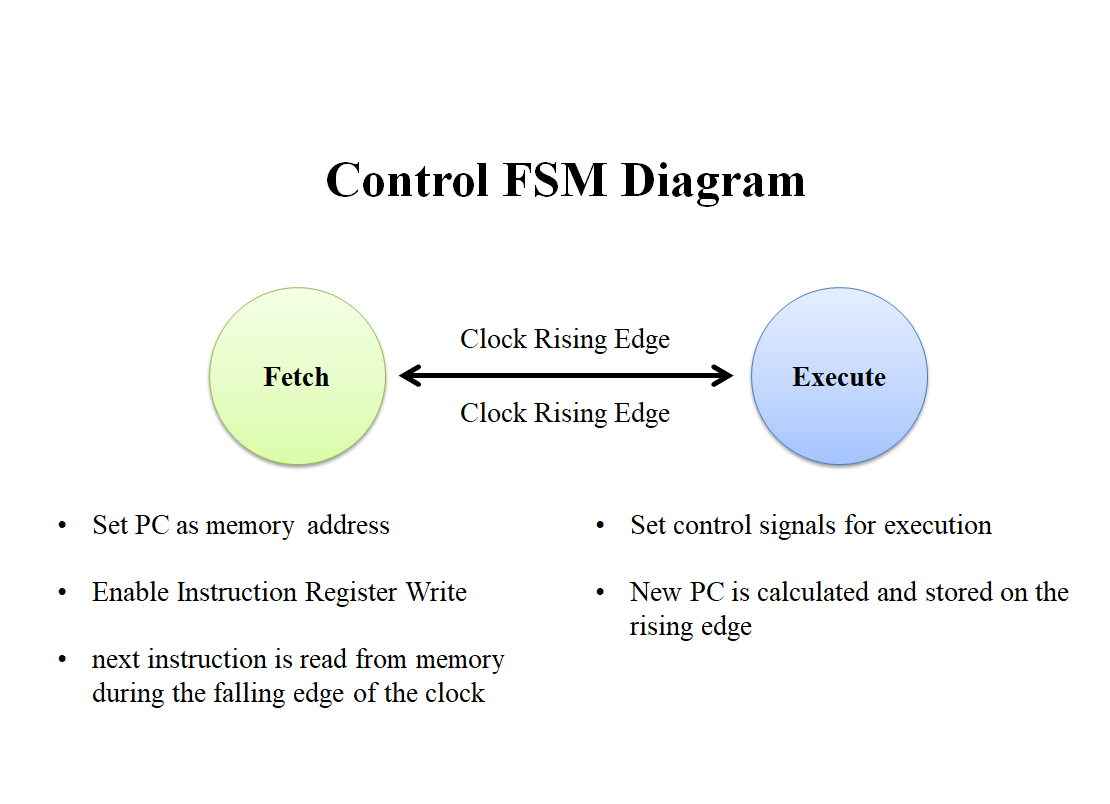
\includegraphics[width=3.4in]{fsm diagram.PNG}
    \caption{Finite state machine diagram of the CPU's control FSM.}
    \label{fig:ctrl_fsm}
  \end{figure}

  The CPU architecture only needs two cycles to execute any instructions. 
  This is accomplished with added parallelism in the data path, and doing 
  negative edge memory reads. 
  An example of the added parallelism in the data path is a dedicated ALU for the 
  program counter, which always produces a PC plus one signal. 
  This is used for the JAL instruction, where the PC plus one signal must be stored 
  in a register at the same time as the new PC is loaded.
\end{document}
